\clearpage
\paragraph{Ex} Försök att diagonalisera $A=\begin{pmatrix}2&4\\4&10\end{pmatrix}$.
\subparagraph{Lösning}
\begin{enumerate}
    \item[Hitta egenvärden:]
        \begin{equation*}
            p(\lambda)=det(A-\lambda I_2)=
            det\begin{pmatrix}
                2-\lambda&4\\4&10-\lambda
            \end{pmatrix}=
            (2-\lambda)(10-\lambda)-16=
            \lambda^2-12\lambda+4
        \end{equation*} 
    \item[Lös ekvationen:]
        \begin{center}
            $p(\lambda)=0$\\
            $\Leftrightarrow (\lambda-6)^2=-4+6^2=32$\\
            $Leftrightarrow \lambda = 6\pm \sqrt{32}=6\pm 4\sqrt{2}$
        \end{center}
    \item[Egenvärden:] \underline{$\lambda=6-4\sqrt{2}$}\\
        $\begin{pmatrix}
            2-6-4\sqrt{2}&4&0\\
            4&10-6-4\sqrt{2}&0
        \end{pmatrix}
        \thicksim
        \begin{pmatrix}
            -4(1-\sqrt{2})&4&0\\
            4&4(1+\sqrt{2})&0
        \end{pmatrix}$\\
        $\thicksim
        \begin{pmatrix}
            -4(1-\sqrt{2})&4&0\\
            4(1-\sqrt{2})&4(1+\sqrt{2})(1-\sqrt{2})&0
        \end{pmatrix}
        \thicksim
        \begin{pmatrix}
            1-\sqrt{2}&-1&0\\
            0&0&0
        \end{pmatrix}$\\
        $\Leftrightarrow\begin{cases}
            (1-\sqrt{2}x=t)\\
            y=t
        \end{cases}
        \Leftrightarrow
        \begin{cases}
            x=t(1+\sqrt{2})
            y=t
        \end{cases}$\\
        Egenvektor till $\lambda=6-4\sqrt{2}$ är $\bm{v}_1=\begin{pmatrix}-1+\sqrt{2}\\1\end{pmatrix}$
        \underline{$\lambda=6+4\sqrt{2}$}\\
        $\begin{pmatrix}
            -4(1+\sqrt{2})&4&0\\
            4&4(1-\sqrt{2})&0
        \end{pmatrix}
        \thicksim
        \begin{pmatrix}
            -4/1+\sqrt{2}&4&0\\
            4(1+\sqrt{2})&4(1-\sqrt{2})(1+\sqrt{2})&0
        \end{pmatrix}$\\
        $\begin{pmatrix}
            1+\sqrt{2}&-1&0\\
            0&0&0
        \end{pmatrix}
        \Leftrightarrow
        \begin{cases}
            (1+\sqrt{2})x=t\\
            y=t
        \end{cases}
        \Leftrightarrow
        \begin{cases}
            x=-(1-\sqrt{2})t\\
            y=t
        \end{cases}$\\
        Egenvektor till $\lambda=6+4\sqrt{2}: \bm{v}_2=\begin{pmatrix}-(1-\sqrt{2})\\1\end{pmatrix}$
\end{enumerate}
Diagonaliseringen av $A$ fås av att låta 
$\bm{v}_1\cdot\bm{v}_2=(\sqrt{2}-1)(\sqrt{2}+1)+1\cdot 1=-1+1=0$
\begin{equation*}
    D=\begin{pmatrix}
        6-4\sqrt{2}&0\\
        0&6+4\sqrt{2}
    \end{pmatrix}\text{, }
    P=\begin{pmatrix}
        \sqrt{2}-1&\sqrt{2}+1\\
        1&1
    \end{pmatrix}
\end{equation*}
\clearpage
\paragraph{Ex} Hitta egenvärden till $A=\begin{pmatrix}
    0&-1&1\\
    -1&-2&-1\\
    1&-1&0
\end{pmatrix}$
\subparagraph{Lösning} $p(\lambda)=det(A-\lambda I_3)=det\begin{pmatrix}
    -\lambda&-1&1\\
    -1&-2-\lambda&-1\\
    1&-1&-\lambda
\end{pmatrix}$\\
\begin{equation*}
    =-\lambda\begin{vmatrix}
        -2-\lambda&-1\\-1&-\lambda
    \end{vmatrix}
    +1\begin{vmatrix}
        -1&-1\\1&-\lambda
    \end{vmatrix}
    +1\begin{vmatrix}
        -1&-2\lambda\\
        1&-1
    \end{vmatrix}
\end{equation*}
\begin{equation*}
    =-\lambda(-(-2-\lambda)\lambda-1)+\lambda+1+1+2+\lambda
    =-\lambda(2\lambda+\lambda^2-1)+2\lambda+4
    =-\lambda^3-2\lambda^2+3\lambda+4
\end{equation*}
Tredjegradspolynom. Svårt.
Om det finns heltalsrötter så delar de den konstanta termen.\\
I detta fall: Möjliga heltalsrötter: $\pm 1,\pm 2, \pm 4$ -1 är en rot!
Vi utför polynomdivision.
Dividera $p(\lambda)=-\lambda^3-2\lambda^2+3\lambda+4$ med $\lambda-(-1)=\lambda+1$.
\begin{equation*}
    -\lambda^3-2\lambda^2+3\lambda+4=-(\lambda+1)(\lambda^2+\lambda-4)
\end{equation*}
Vi löser nu:
\begin{equation*}
    \lambda^2+\lambda-4=0
    \Leftrightarrow
    (\lambda+\frac{1}{2})^2=4+\frac{1}{4}=\frac{17}{4}
    \Leftrightarrow
    -\frac{1}{2}\pm \frac{\sqrt{17}}{4}
\end{equation*}

\chapter{Grafer (Avs 9.1)}

\paragraph{Definition} En graf $G$ består av två mängder $G=(V,E)$ där $V$ är 
\underline{noder} och $E$ är \underline{kanter} mellan noderna.


\paragraph{Ex} $V=\{1,2,3\}$\indent$E=\{\{1,2\},\{1,3\}\}$\\
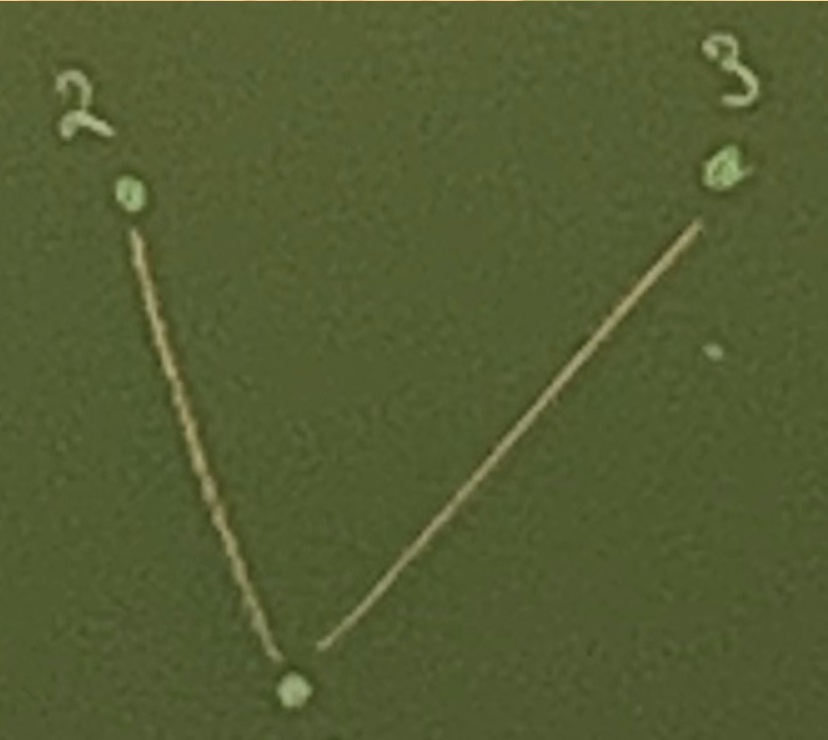
\includegraphics[scale=0.25]{imgs/img01.png}

\paragraph{Definition} \underline{Graden} av en nod $v$ är antalet kanter med noden, $d(v)$.

\paragraph{Definition} En riktad graf $G$ består av två mängder $G=(V,E)$ där $V$ är noder och $E$ är kanter.
Nu är $E$ en mängd av ordnade par av noder.

\paragraph{Ex} $V=\{1,2,3,4\}$\indent$E=\{(1,2),(2,4),(4,3),(3,4),(1,3)\}$\\
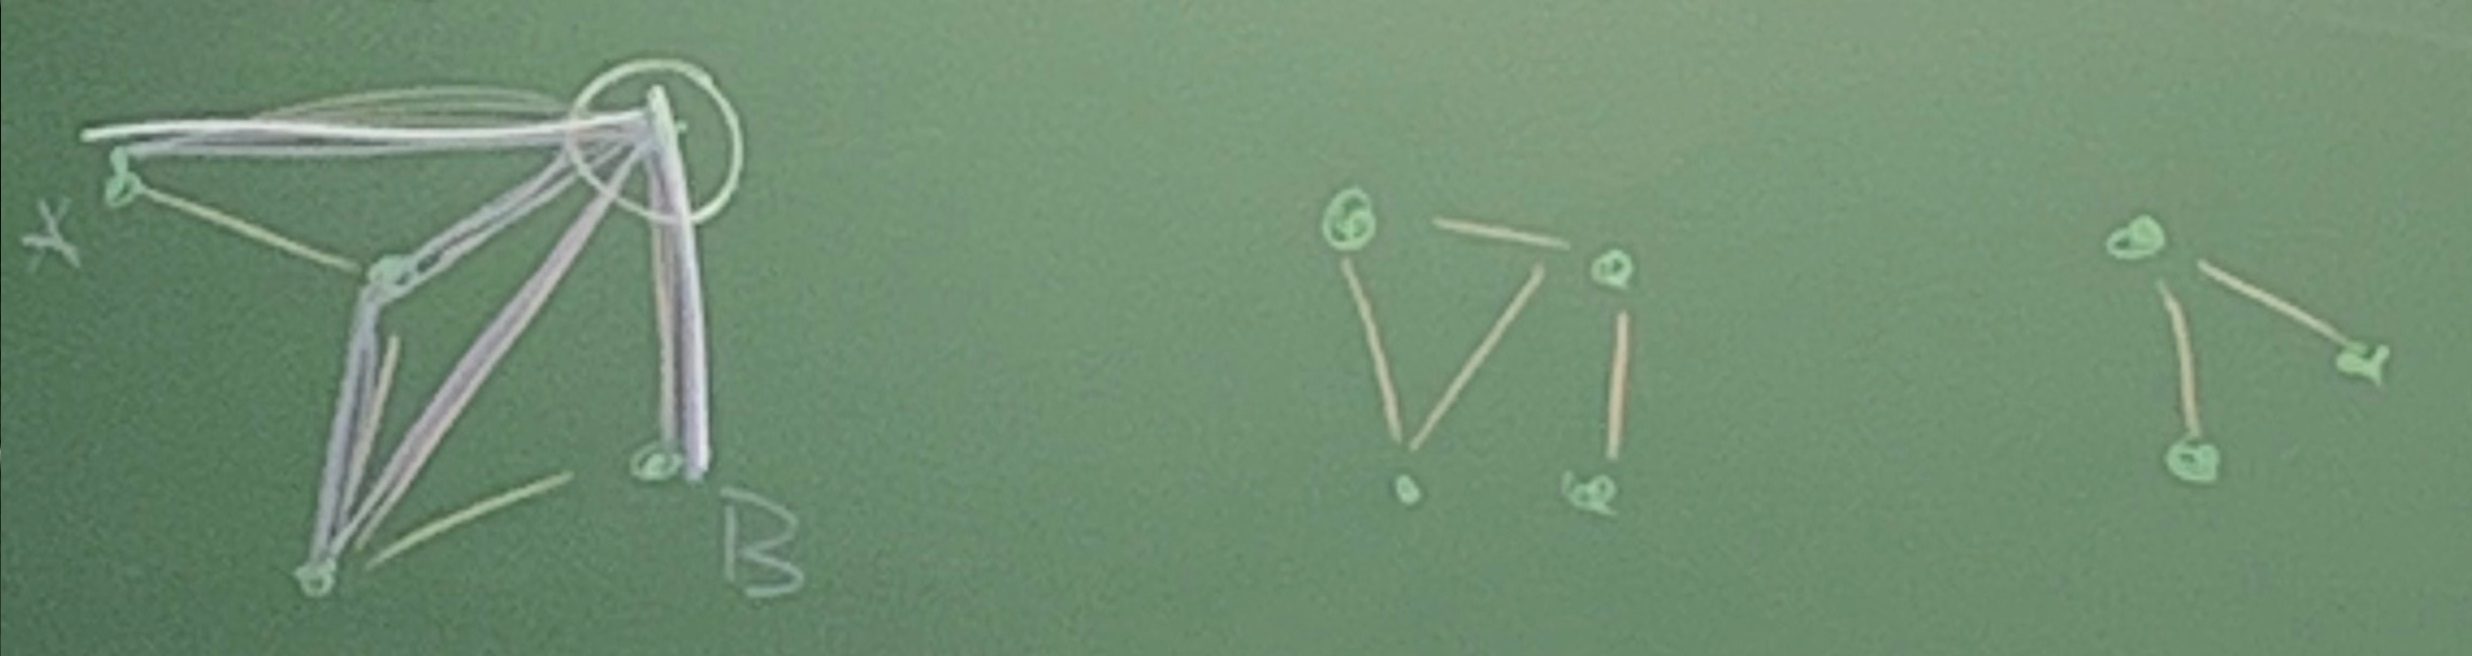
\includegraphics[scale=0.13]{imgs/img02.png}
I riktade grafer har kanter en start- och slutnod.

\paragraph{Definition} En \underline{väg av längd $k$} mellan nod $A$ och $B$ är en lista av kanter $\bm{e}_1,\bm{e}_2,\ldots,\bm{e}_k$ där $A\in\bm{e}_1$ och $B\in\bm{e}_k$.
\begin{itemize}
    \item Vägen sägs vara \underline{enkel} om varje nod finns i högst två av kanterna i listan.
    \item Om $A=B$ då kallas vägen en $cykel$.
    \item Om det finns en väg mellan alla noder då sägs grafen vara \underline{sammanhängande}
\end{itemize}

\paragraph{Sats 9.14} Om det finns en väg mellan två noder då finns det en enkel väg.

\paragraph{Sats 9.15} Om en graf har $n$ noder då har en enkel väg högst $n$ kanter.

\chapter{Grannmatriser (Avs 9.2)}

\paragraph{Definition} Om $G=(V,E)$ är en graf med $n$ noder då ges \underline{grannmatrisen till $G$} av $n\times n$-matrisen $A$ som på plats $(i,j)$ ges av $a_{i,j}=\left\lbrace\begin{matrix}1\\0\end{matrix}\right.$, $\{i,j\}\in E$ annars.
Om $G$ är en riktad graf ges grannmatrisen $A$ av den matris som på plats $(i,j)$ är $a_{i,j}=\left\lbrace\begin{matrix}1\\0\end{matrix}\right.$, $a_{i,j}\in E$ annrs.

\paragraph{Ex}
$A=\begin{pmatrix}
    0&1&1\\
    1&0&0\\
    1&0&0
\end{pmatrix}
\text{\hspace{20px}}
A=\begin{pmatrix}
    0&1&0\\
    0&0&0\\
    1&0&0
\end{pmatrix}$\\
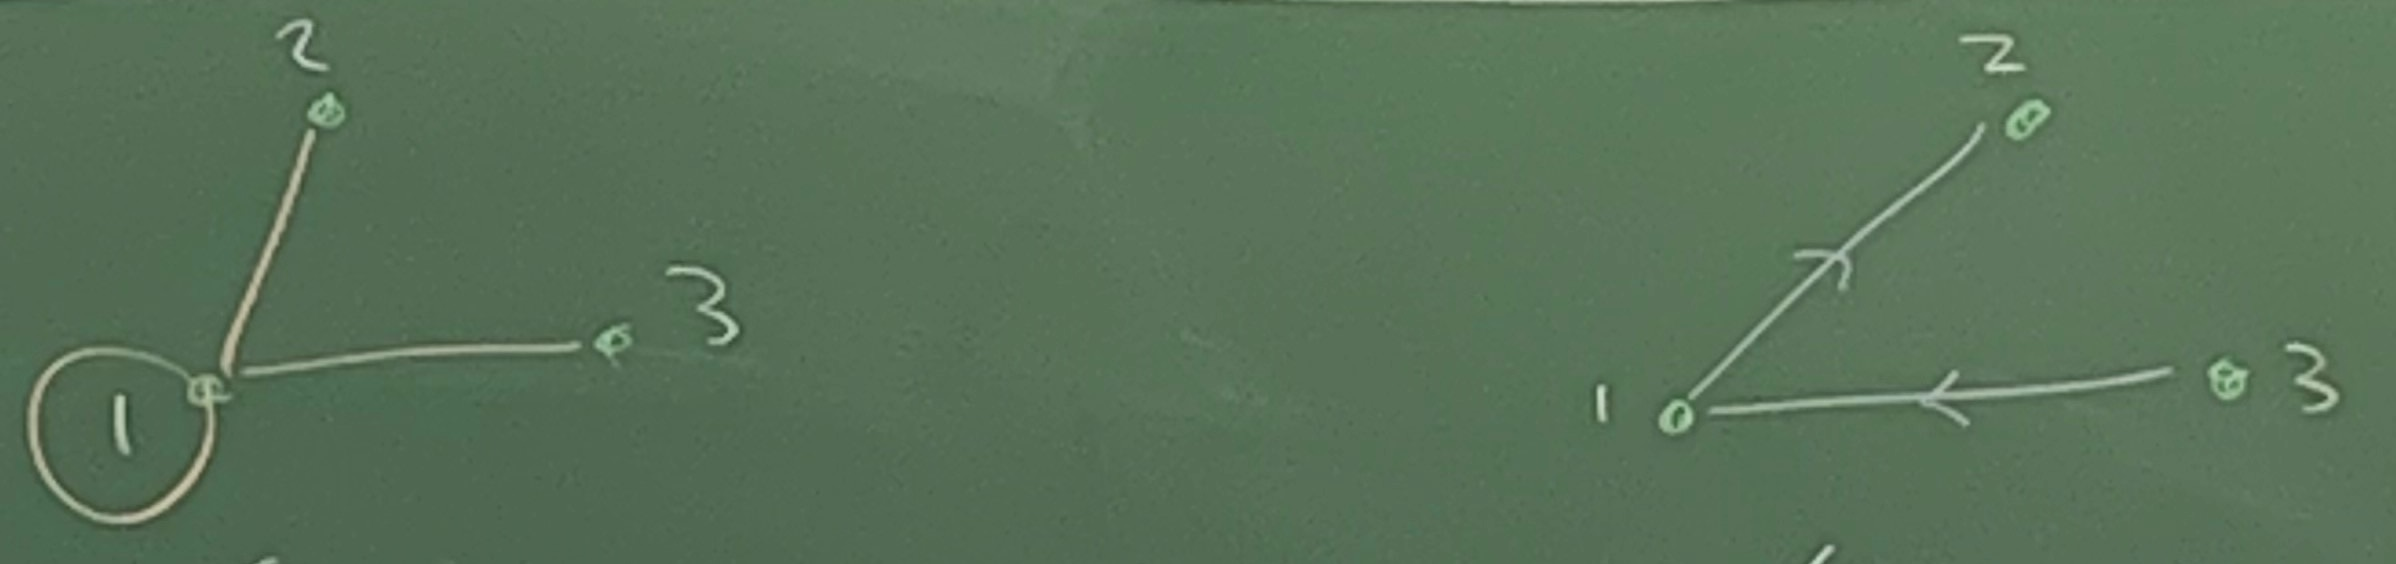
\includegraphics[scale=0.14]{imgs/img03.png}

\paragraph{Sats 9.19} Om $A$ är grannmatrisen till en graf då är elementet på plats $(i,j)$ i $A^k$ är antalet vägar av längd $k$ från nod $i$ till nod $j$.

\paragraph{Följdsats 9.20} Det finns en väg från nod $i$ till nod $j \Leftrightarrow$ element $(i,j)$ i $A^k$ inte är noll för något $k$

\paragraph{Sats 9.21} Det finns en väg från nod $i$ till nod $j \Leftrightarrow$ element $(i,j)$ i $\sum^n_{k=1}A^k$ inte är noll.

\paragraph{Följdsats 9.22} Grafen $G$ är sammanhängande $\Leftrightarrow$ Varje element i $\sum^n_{k=1}A^k$ är nollskilt.

\chapter{Slumpvandringar på grafer (Avs 9.3)}
Antag att vi har en graf $G=(V,E)$ och att vi startar i någon nod $v$.
Vi går till en nod som har en kant med $v$ med sannolikhet $\frac{1}{d(v)}$.
Fortsätter vi såhär får vi en så kallad \underline{slumpvandring}.

\paragraph{Definition} Givet en grannmatris $A$ låter vi $M$ vara den matris som på plats $(i,j)$ ges av:
\begin{equation*}
    m_{i,j}=\frac{a_{i,j}}{\sum^n_{k=1}a_{i,k}}
\end{equation*}
Det här kommer att ge att $m_{i,1}+m_{i,2}+\ldots+m_{i,n}=1$

\paragraph{Sats 9.27} Element $(i,j)$ i $M^k$ det är sannolikheten att vi befinner oss i nod $j$ om vi började i nod $i$ om vi har tagit $k$ steg.
\\\\
Om $\bm{x}^t$ är en radvekter med positiva element vars summa är $I$ kallas $\bm{x}^t$ för en \underline{fördelningsvektor}.
Detta ska tolkas som att $\bm{x}^t=\begin{pmatrix}
    x_1&x_2&\ldots&x_n
\end{pmatrix}$, vi startar på nod $i$ med sannolikhet $x_i$

\paragraph{Sats 9.27 (forts.)} Uttrycket $\bm{x}^tM^k$ är sannolikheten att vi befinner oss i en viss nod efter $k$ steg.